% Template for Cogsci submission with R Markdown

% Stuff changed from original Markdown PLOS Template
\documentclass[10pt, letterpaper]{article}

\usepackage{cogsci}
\usepackage{pslatex}
\usepackage{float}
\usepackage{caption}

% amsmath package, useful for mathematical formulas
\usepackage{amsmath}

% amssymb package, useful for mathematical symbols
\usepackage{amssymb}

% hyperref package, useful for hyperlinks
\usepackage{hyperref}

% graphicx package, useful for including eps and pdf graphics
% include graphics with the command \includegraphics
\usepackage{graphicx}

% Sweave(-like)
\usepackage{fancyvrb}
\DefineVerbatimEnvironment{Sinput}{Verbatim}{fontshape=sl}
\DefineVerbatimEnvironment{Soutput}{Verbatim}{}
\DefineVerbatimEnvironment{Scode}{Verbatim}{fontshape=sl}
\newenvironment{Schunk}{}{}
\DefineVerbatimEnvironment{Code}{Verbatim}{}
\DefineVerbatimEnvironment{CodeInput}{Verbatim}{fontshape=sl}
\DefineVerbatimEnvironment{CodeOutput}{Verbatim}{}
\newenvironment{CodeChunk}{}{}

% cite package, to clean up citations in the main text. Do not remove.
\usepackage{apacite}

% KM added 1/4/18 to allow control of blind submission


\usepackage{color}

% Use doublespacing - comment out for single spacing
%\usepackage{setspace}
%\doublespacing


% % Text layout
% \topmargin 0.0cm
% \oddsidemargin 0.5cm
% \evensidemargin 0.5cm
% \textwidth 16cm
% \textheight 21cm

\title{Children social information seeking during familiar and novel language
processing}

\usepackage{threeparttable}
\usepackage{booktabs}

\author{{\large \bf Kyle MacDonald (kemacdonald@ucla.edu)} \\ Department of Communication, UCLA  \AND {\large \bf Elizabeth Swanson (elizswan@stanford.edu)} \\ Department of Psychology, Stanford University  \AND {\large \bf Michael C. Frank (mcfrank@stanford.edu)} \\ Department of Psychology, Stanford University  }

\begin{document}

\maketitle

\begin{abstract}
Children process language in complex environments where there are often
many things to talk about. How do they understand and learn words
despite this noisy input? Statistical learning accounts emphasize that
children can aggregate consistent word-object co-occurrences across
multiple labeling events to reduce uncertainty over time.
Social-pragmatic theories argue that language is acquired within
interactions with social partners who can reduce ambiguity within
individual labeling events. Here, we present three eye-tracking studies
that ask how children integrate statistical and social information to
seek information during real-time language processing. First, children
and adults did not delay their gaze shifts to gather a post-nominal
social cue to reference (another speaker's eye gaze). Second, when
processing novel words adults fixated more on a speaker who provided a
disambiguating gaze and showed stronger recall for word-object links
learned via the social cue. Finally, in contrast to the familiar word
context, children and adults fixated longer on a speaker who produced a
gaze cue when labeling novel objects, which, in turn, led to increased
looking to the named object and less looking to the other objects in the
scene. Moreover, children, but not adults, increased their looking to
the interlocutor throughout the experiment. Together, these results
suggest that learners flexibly integrate their knowledge of object
labels to decide whether to seek social information, which then shapes
the information that comes into contact with statistical learning
mechanisms.

\textbf{Keywords:}
eye movements; language processing; information-seeking; word learning;
gaze following
\end{abstract}

\hypertarget{introduction}{%
\section{Introduction}\label{introduction}}

How is it that children, who are just learning how to walk, can segment
units from a continuous stream of linguistic information and map them to
their corresponding conceptual representations. Children's
word-to-meaning mapping skill becomes even more striking when we
consider that a speaker's intended meaning is mostly unconstrained by
the co-occurring context; a point made famous by W.V. Quine's example of
a field linguist trying to select the target meaning of a new word
(``gavagai'') from the set of possible meanings consistent with the
event of a rabbit running (e.g., ``white,'' ``rabbit,'' ``dinner,''
etc.) (Quine 1960).

Research on early lexical development has pursued several solutions to
the problem of referential uncertainty. First, lab-based studies and
computational models have explored how children's statistical learning
mechanisms can reduce ambiguity during word learning. Under these
\emph{cross-situational} learning accounts, learners can overcome
referential uncertainty within a specific labeling event by tracking the
elements of a context that remain consistent across multiple exposures
to a new word (Yu and Smith 2007; Siskind 1996; Roy and Pentland 2002).
Experiments with 12-month-old infants find that they are capable of
learning novel words via repeated exposures to consistent word-object
pairings (Smith and Yu 2008). Moreover, simulation studies show that
models of a simple cross-situational learner can acquire an adult-sized
vocabulary from exposures that fall well within the bounds of children's
language experience (Blythe, Smith, and Smith 2010) and even when
referential uncertainty is high (Blythe, Smith, and Smith 2016).

Social-pragmatic theories argue that children's social partners can
reduce the complexity of the learning task (Clark 2009; Bloom 2002;
Hollich et al. 2000). For example, observational studies show that
adults are skilled at using gesture and eye gaze to coordinate language
interactions with children (Estigarribia and Clark 2007). Moreover, from
a young age, children can use a speaker's gaze to infer intended word
meanings (Baldwin 1993) and lab-based experiments with adults show that
following gaze reduces the cognitive load associated with processing
linguistic reference (Sekicki and Staudte 2018). Finally, correlational
studies have demonstrated links between children's early gaze following
skill and later vocabulary growth (Brooks and Meltzoff 2005; Carpenter
et al. 1998), suggesting that seeking the direction of another's gaze
can facilitate language processing.

Thus, both social and statistical information can reduce children's
uncertainty about reference during language processing. These processes,
however, are unlikely to operate in isolation, and a sophisticated
learner could integrate the two sources of information to facilitate
acquisition. Several computational models of word learning have pursued
integrative accounts of social and statistical learning. For example,
work by Yu and Ballard (2007) found better word-object mapping
performance if their model used social cues (e.g., eye gaze) to increase
the strength of specific word-object associations stored from a given
labeling event. Moreover, Frank, Goodman, and Tenenbaum (2009) showed
that adding social inferences about a speaker's intended meaning to a
word learning model captured a variety of key behavioral findings in
early language development (e.g., mutual exclusivity and the use of gaze
to disambiguate reference).

The statistical and social accounts of word learning reflect a somewhat
passive construal of the learner. Children, however, can exert control
over the environment via actions such as choosing where to look,
pointing, and asking verbal questions. A body of research outside the
domain of language acquisition shows that active control can speed
learning because it allows people to use their prior knowledge and
current uncertainty to seek more useful information (e.g., asking a
question about something that is particularly confusing) (Gureckis and
Markant 2012; Settles 2012; Castro et al. 2009). Moreover, recent
empirical and modeling work has begun to explore the role of active
control in word learning (Partridge et al. 2015; Hidaka, Torii, and
Kachergis 2017). For example, Kachergis, Yu, and Shiffrin (2013) showed
that adults who were able to select the set of novel objects that would
be labeled learned more than adults who passively experienced the
word-object pairings generated by the experiment.

In the current paper, we pursue the idea that children flexibly seek
information from social partners to support language processing. We
focus on children's eye movements as a case study of highly practiced
information seeking behavior available to the young learner. Visual
fixations are also crucial for the task of grounded language processing,
which involves linking the linguistic signal to the visual world using
information gathered through decisions about where to direct gaze.
Moreover, recent work has shown that infants' ability to sustain visual
attention on objects is a strong predictor of their novel word learning
(Smith and Yu 2013) and social partners can facilitate this form of
sustained attention (Yu and Smith 2016). Taken together, these findings
suggest that real-time selection of visual information is a good case
study to explore how children integrate social and statistical during
language processing.

\hypertarget{current-studies}{%
\subsection{Current studies}\label{current-studies}}

The current studies synthesize ideas from social, statistical, and
active learning. We ask how children's real-time information selection
via eye movements is shaped by social information present in the
labeling moment and by statistical information about word-object links
that is accumulated over a longer timescale. We draw on ideas from
theories of goal-based vision that characterize eye movements as
information seeking decisions that aim to minimize uncertainty about the
world (Hayhoe and Ballard 2005). Under this account, learners should
integrate statistical and social information by considering the
usefulness (i.e., information gained) of an eye movement for their
current task goal.

The studies are designed to answer several open questions in early
language processing. First, how do statistical learning mechanisms
operate over social input? Most prior work on statistical word learning
has used linguistic stimuli that come from a disembodied voice, removing
a rich set of multimodal cues (e.g., gestures, facial expressions, mouth
movements) that occur during face-to-face communication. By including a
social fixation target, we can ask how social contexts shape the input
to statistical word learning mechanisms.

Second, how do children seek visual information to support their
language processing? We characterize eye movements as decisions under
uncertainty and time constraints. Using this theoretical framework
allows us to bring top-down, goal-based models of vision (Hayhoe and
Ballard 2005) into contact with work on language-driven eye movements
(Allopenna, Magnuson, and Tanenhaus 1998) that typically characterize
gaze shifts as the output of the language comprehension process.

Finally, this study asks how children's in-the-moment decisions connect
to learning over a longer timescale. Following McMurray, Horst, and
Samuelson (2012), we separate situation-time behaviors (figuring out the
referent of a word) from developmental-time processes (building a stable
mapping between a word and concept). Moreover, by studying changes in
patterns of eye movements throughout learning, we add to a recent body
of empirical work that emphasizes the importance of linking real-time
information selection to longer-term statistical learning (Yu and Smith
2012).

\hypertarget{analytic-approach}{%
\section{Analytic approach}\label{analytic-approach}}

To quantify evidence for our predictions, we present analyses of (1) the
time course of listeners' looking to each area of interest (AOI) and (2)
the Reaction Time (RT) and Accuracy of listeners' first shifts away from
the speaker's face and to the objects.

First, we analyzed the time course of participants' looking to each AOI
in the visual scene as the target sentence unfolded. Proportion looking
reflects the mean proportion of trials on which participants fixated on
the speaker, the target image, or the distracter image at every 33-ms
interval of the stimulus sentence. We tested condition differences in
the proportion looking to the language source -- signer or speaker --
using a nonparametric cluster-based permutation analysis, which accounts
for the issue of taking multiple comparisons across many time bins in
the timecourse (Maris and Oostenveld 2007). A higher proportion of
looking to the language source in the gaze condition would indicate
listeners' prioritization of seeking visual information from the
speaker.

Next, we analyzed the RT and Accuracy of participants' initial gaze
shifts away from the speaker to objects. RT corresponds to the latency
of shifting gaze away from the central stimulus to either object
measured from the onset of the target noun. All reaction time
distributions were trimmed to between zero and two seconds, and RTs were
modeled in log space. Accuracy corresponds to whether participants'
first gaze shift landed on the target or the distracter object. While we
use the term ``accuracy'' as a label for this dependent measure in our
task, we do not want to claim that fixations to the distracter object
are incorrect in a general sense since these behaviors could be useful
for other goals such as better encoding the objects in the scene. If
listeners generate slower but more accurate gaze shifts, this provides
evidence that gathering more visual information from the speaker led to
more robust language processing in the gaze context.

In Experiments 2 and 3, which measure novel word learning as a function
of multiple word-object exposures, we compute proportion looking to the
speaker for each trial, which corresponds to the amount of time looking
to the speaker over the total amount of time looking at the three AOIs.
We interpret a higher looking to the speaker as increased information
seeking to gather the social cue. We also compute the proportion looking
to the target object, which corresponds to the time spent looking to the
target over the total amount of time fixating on both the target and the
distracter objects. We interpret higher target looking on exposure
trials with gaze cues indicate that learners followed the gaze cue. We
interpret higher target looking on test trials indicates stronger
retention for the newly learned word-object links. In all analyses of
learning, we treat trial number as a continuous variable and age group
-- children vs.~adults -- as categorical.

We used the \texttt{brms} (Bürkner 2017) package to fit Bayesian
mixed-effects regression models. The mixed-effects approach allowed us
to model the nested structure of our data -- multiple trials for each
participant and item, and the within-participants manipulation used in
Experiments 1 and 3. We used Bayesian estimation to quantify uncertainty
in our point estimates, which we communicate using a 95\% Highest
Density Interval (HDI), providing a range of credible values given the
data and model.

\hypertarget{experiment-1}{%
\section{Experiment 1}\label{experiment-1}}

In Experiment 1, we measured the time course of children and adults'
decisions about visual fixation as they processed sentences with
familiar words (e.g., ``Where's the ball?'').\footnote{See
  \url{https://osf.io/2q4gw/} for a pre-registration of the analysis
  plan.} We manipulated whether the speaker also produced a post-nominal
gaze cue to the named object. The visual world consisted of three
fixation targets (a center video of a person speaking, a target picture,
and a distracter picture; see Figure 1). The primary question of
interest is whether listeners would delay shifting their looking away
from the speaker's face when she was likely to generate a gaze cue. We
predicted that choosing to fixate longer on the speaker would allow
listeners to gather more language-relevant visual information and
facilitate comprehension. In contrast, if listeners show parallel gaze
dynamics across the gaze and no-gaze conditions, this pattern suggests
that hearing the familiar word was the primary factor driving shifts in
visual attention.

\hypertarget{methods}{%
\subsection{Methods}\label{methods}}

\hypertarget{participants}{%
\subsubsection{Participants}\label{participants}}

\begin{table}[tbp]
\begin{center}
\begin{threeparttable}
\caption{\label{tab:make-ss-table}Age distributions of children in Experiments 1 and 2. All ages are reported in months.}
\begin{tabular}{lllll}
\toprule
Experiment & \multicolumn{1}{c}{n} & \multicolumn{1}{c}{Mean} & \multicolumn{1}{c}{Min} & \multicolumn{1}{c}{Max}\\
\midrule
Exp. 1 (familiar words) & 38 & 55.50 & 35.60 & 71.04\\
Exp. 2 (novel words) & 54 & 52.60 & 36.26 & 70.94\\
\bottomrule
\end{tabular}
\end{threeparttable}
\end{center}
\end{table}

Participants were native, monolingual English-learning children (\(n=\)
38; 19 F) and adults (\(n=\) 33; 23 F). All participants had no reported
history of developmental or language delay and normal vision. 12
participants (9 children, 3 adults) were run but not included in the
analysis because either the eye tracker falied to calibrate (8 children,
2 adults) or the participant did not complete the task (1 children, 1
adults).

\hypertarget{materials}{%
\subsubsection{Materials}\label{materials}}

\emph{Linguistic stimuli.} The video/audio stimuli were recorded in a
sound-proof room and featured two female speakers who used natural
child-directed speech and said one of two phrases: ``Hey! Can you find
the (target word)'' or "Look! Where's the (target word). The target
words were: ball, bunny, boat, bottle, cookie, juice, chicken, and shoe.
The target words varied in length (shortest = 411.68 ms, longest =
779.62 ms) with an average length of 586.71 ms.

\emph{Gaze manipulation}. To create the stimuli in the gaze condition,
the speaker waited until she finished producing the target sentence and
then turned her head to gaze at the bottom right corner of the camera
frame. After looking at the named object, she then returned her gaze to
the center of the frame. We chose to allow the length of the gaze cue to
vary to keep the stimuli naturalistic. The average length of gaze was
2.12 seconds with a range from 1.78 to 3.07 seconds.

\emph{Visual stimuli.} The image set consisted of colorful digitized
pictures of objects presented in fixed pairs with no phonological
overlap between the target and the distracter image (cookie-bottle,
boat-juice, bunny-chicken, shoe-ball). The side of the target picture
was counterbalanced across trials.

\hypertarget{procedure}{%
\subsubsection{Procedure}\label{procedure}}

\begin{CodeChunk}
\begin{figure*}[t]

{\centering 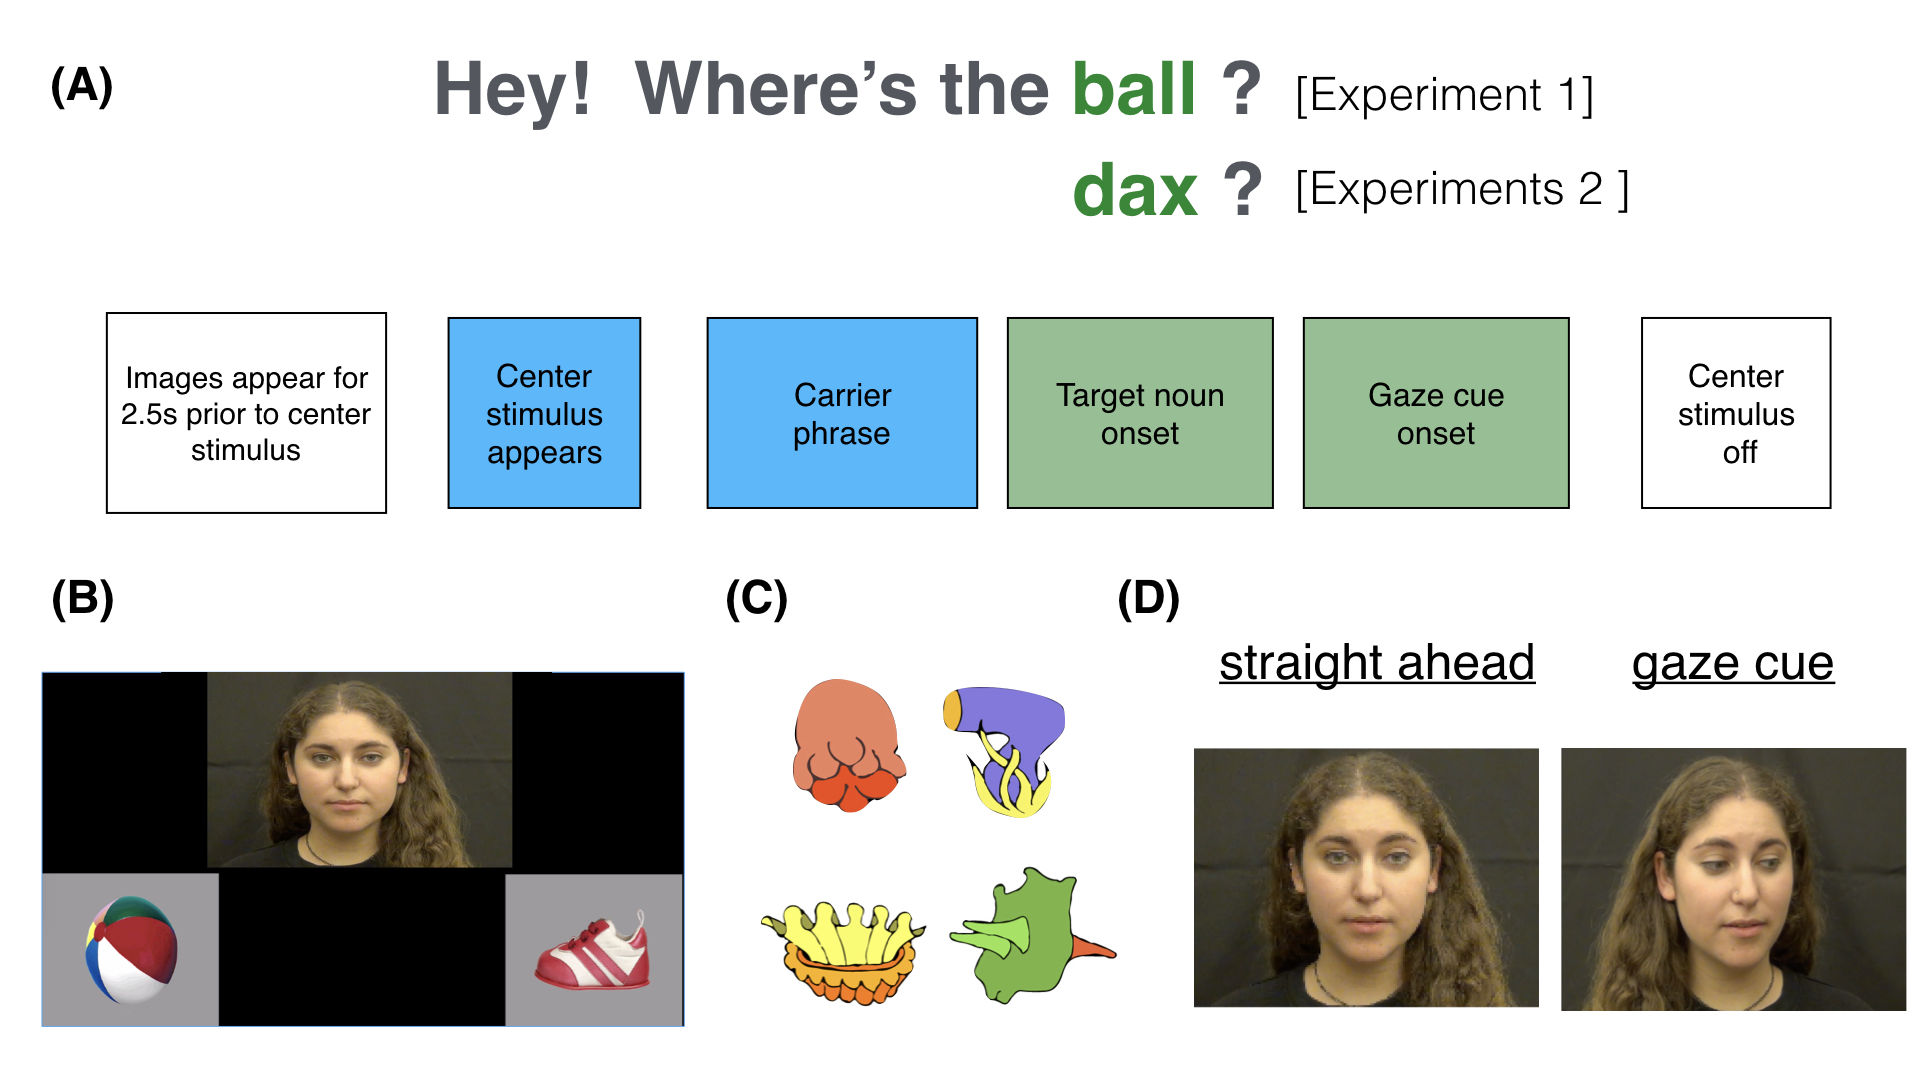
\includegraphics[width=0.7\linewidth]{/Users/kylemacdonald/Documents/Projects/SPEED-ACC-NOVEL/writing/figures/plots/gaze_stimuli} 

}

\caption[Stimuli for Experiments 1 and 2]{Stimuli for Experiments 1 and 2. Panel A shows the structure of the linguistic stimuli for a single trial. Panel B shows the layout of the fixation locations for all tasks: the center stimulus, the target, and the distracter. Panel C shows a sample of the images used as novel objects in Experiment 2. Panel D shows an example of the social gaze manipulation.}\label{fig:gaze-stimuli}
\end{figure*}
\end{CodeChunk}

Participants viewed the task on a screen while their gaze was tracked
using an SMI RED corneal-reflection eye-tracker mounted on an LCD
monitor, sampling at 30 Hz. The eye-tracker was first calibrated for
each participant using a 6-point calibration. On each trial,
participants saw two images of familiar objects on the screen for two
seconds before the center stimulus appeared. Next, they processed the
target sentence -- which consisted of a carrier phrase, a target noun,
and a question -- followed by two seconds without language to allow for
a response. Both children and adults saw 32 trials (16 gaze trials; 16
no-gaze trials) with several filler trials interspersed to maintain
interest. The gaze manipulation was presented in a blocked design with
the order of block counterbalanced across participants.

\hypertarget{results-and-discussion}{%
\subsection{Results and Discussion}\label{results-and-discussion}}

\emph{Timecourse looking.} We first analyzed how the presence of gaze
influenced listeners' distribution of attention across the three
fixation locations while processing familiar words. At target-noun
onset, listeners tended to look more at the speaker than the objects. As
the target noun unfolded, the mean proportion looking to the center
decreased as participants shifted their gaze to the images. Proportion
looking to the target increased sooner and reached a higher asymptote
compared to proportion looking to the distracter for both gaze
conditions with adults spending more time looking at the target compared
to children. After looking to the named referent, listeners tended to
shift their gaze back to the speaker's face.

\begin{CodeChunk}
\begin{figure*}[t]

{\centering 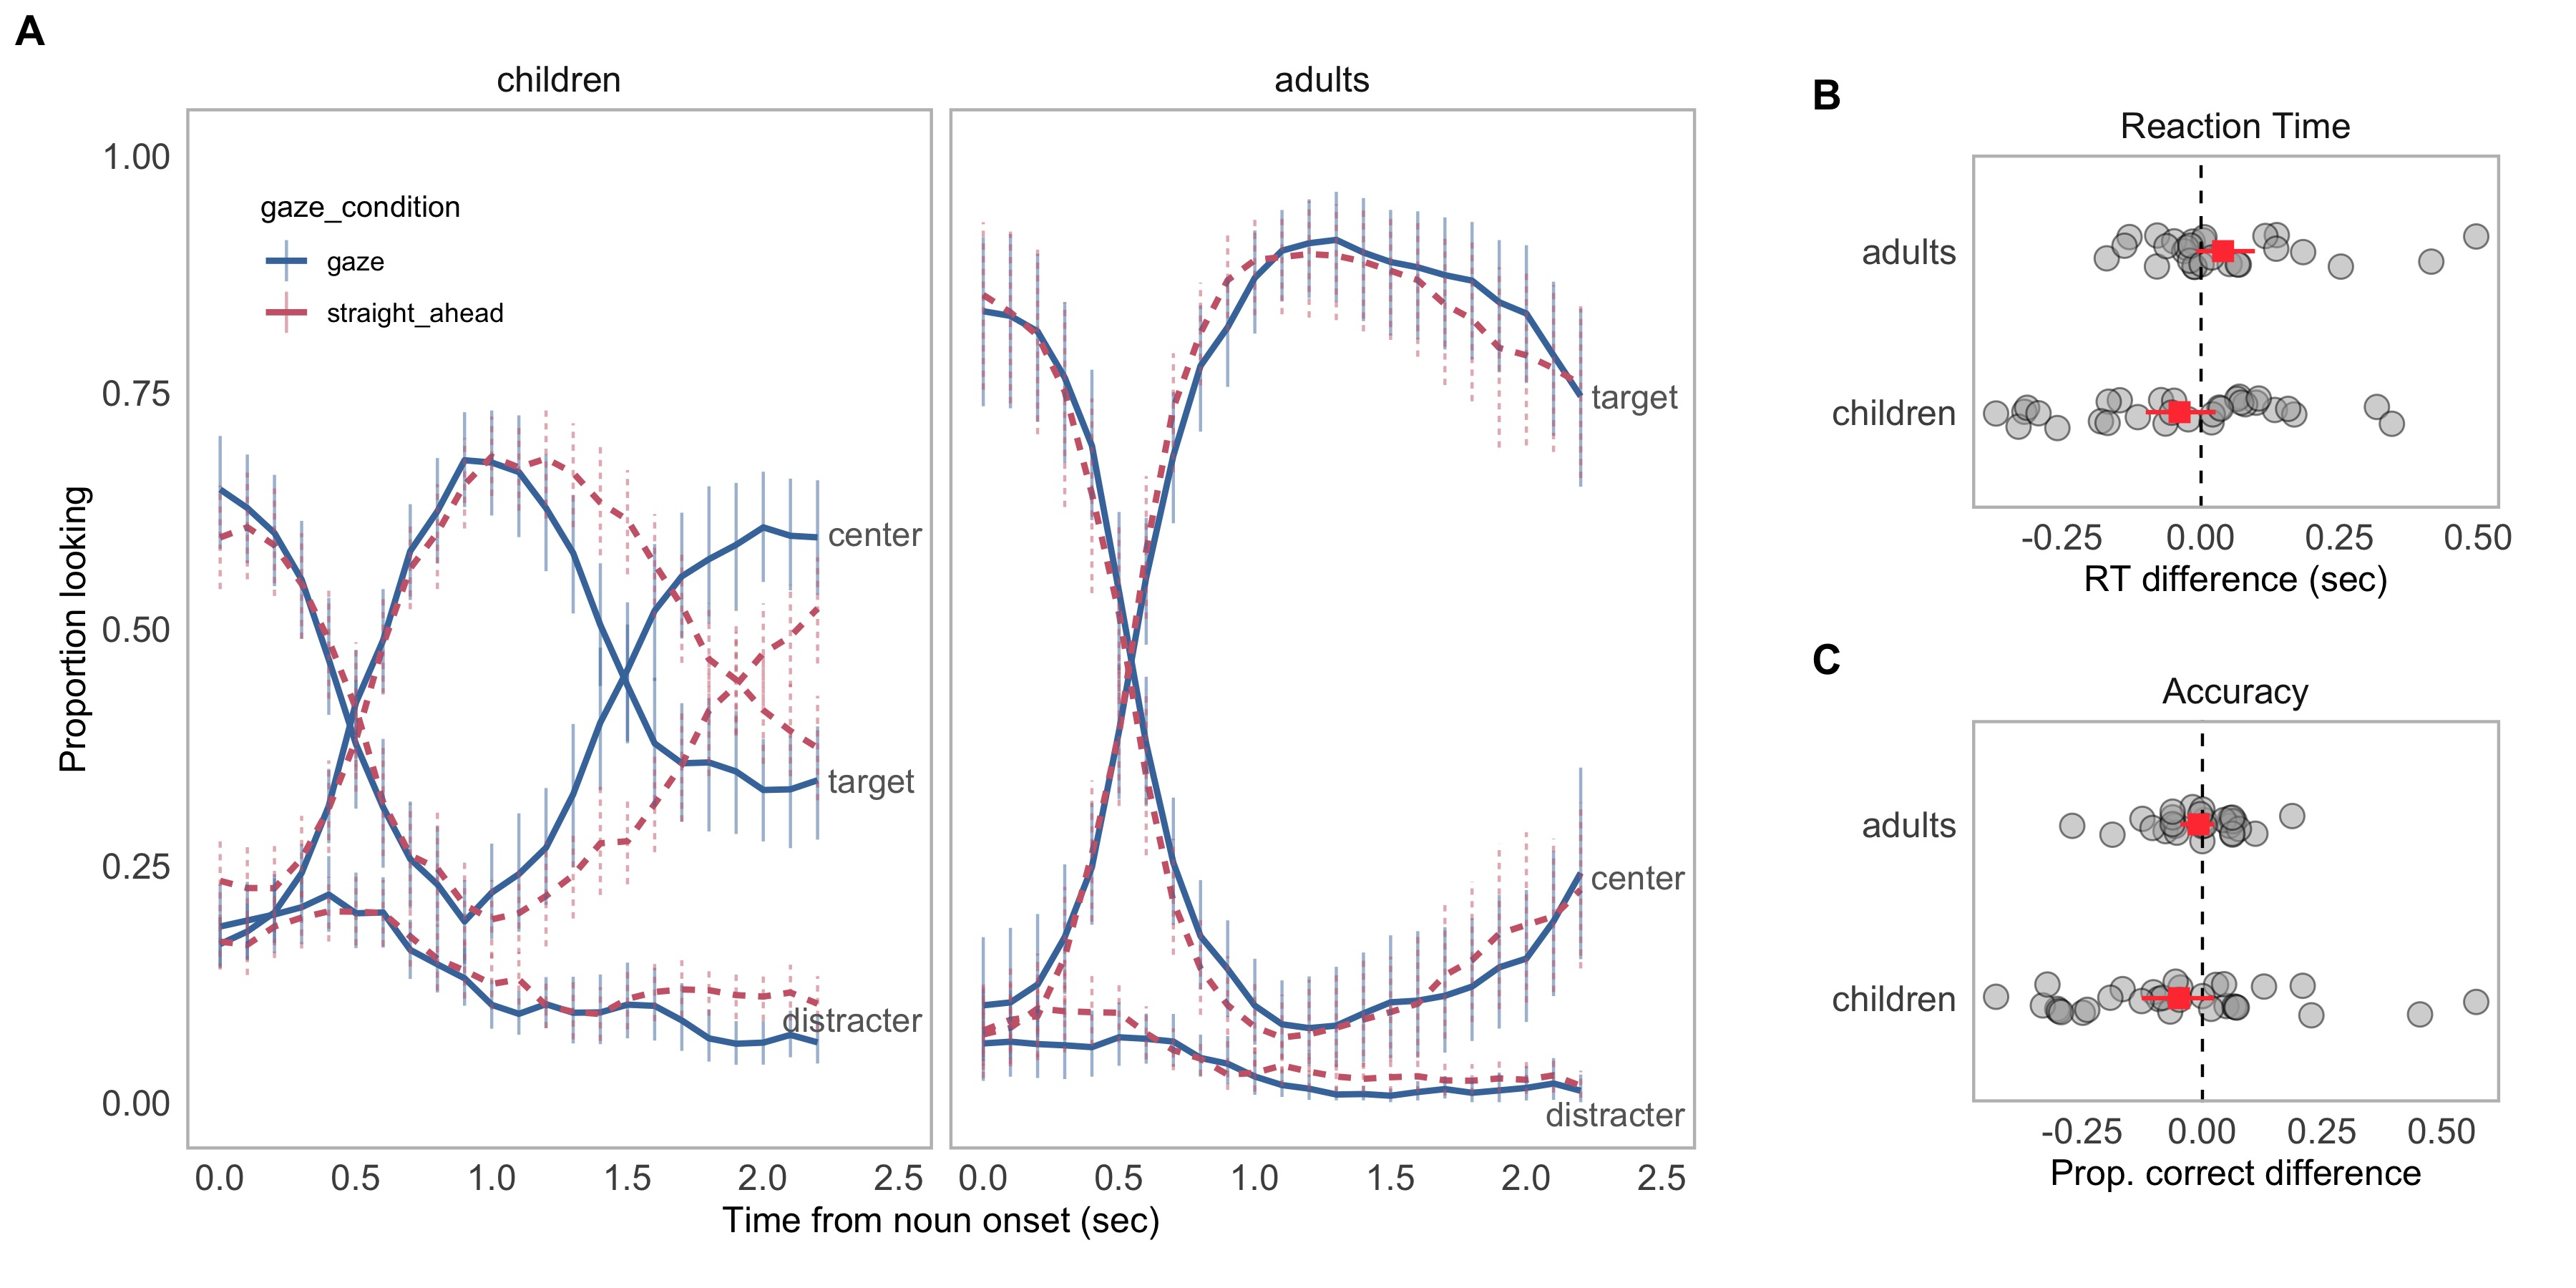
\includegraphics[width=0.85\linewidth]{/Users/kylemacdonald/Documents/Projects/SPEED-ACC-NOVEL/writing/figures/plots/speed_acc_fam_behav} 

}

\caption[Timecourse looking, first shift Reaction Time (RT), and Accuracy results for children and adults in Experiment 1]{Timecourse looking, first shift Reaction Time (RT), and Accuracy results for children and adults in Experiment 1. Panel A shows the overall looking to the center, target, and distracter stimulus for each gaze condition and age group. Panel B shows the distribution of pairwise contrasts between each participant's RT in the gaze and no-gaze conditions. The square point represents the group means. The vertical dashed line represents the null model of zero condition difference. Error bars represent the 95\% HDI. Panel C shows the same information but for first shift accuracy.}\label{fig:speed-acc-gaze-results}
\end{figure*}
\end{CodeChunk}

We did not see evidence that the presence of a post-nominal gaze cue
changed how children or adults allocated attention early in the target
word. Children in the gaze condition, however, tended to shift their
focus back to the speaker earlier after shifting gaze to the named
object and spent more time fixating on the speaker's face throughout the
rest of the trial (\(p < .001\); nonparametric cluster-based permutation
analysis). Next, we ask how these different processing contexts changed
the timing and accuracy of children's initial decisions to shift away
from the center stimulus.

\emph{First shift RT and Accuracy.} To quantify differences across the
groups, we fit a Bayesian linear mixed-effects regression predicting
first shift RT as a function of gaze condition and age group:
\emph{Log(RT) \(\sim\) gaze condition + age group + (gaze\_condition +
item \textbar{} subject)}. Both children and adults generated similar
RTs in the gaze (children \(M_{rt}\) = 563.159 ms, adults \(M_{rt}\) =
652.405 ms) and no-gaze (children \(M_{rt}\) = 575.762 ms, adults
\(M_{rt}\) = 608.314 ms) conditions, with the null value of zero
condition differences falling within the 95\% credible interval
(\(\beta\) = -0.36, 95\% HDI {[}-0.89, 0.06{]}). Next, we fit the same
model to estimate first shift accuracy. Adults generated more accurate
gaze shifts (\(M\) = 0.9) compared to children (\(M\) = 0.64) with the
null value falling outside the 95\% HDI (\(\beta_{age}\) = -1.76, 95\%
HDI {[}-2.19, -1.34{]}). Similar to the RT analysis, we did not find
strong evidence of a difference in performance across the gaze
conditions (\(\beta\) = 0.10, 95\% HDI {[}-0.18, 0.41{]}).

Taken together, the time course and first shift analyses suggest that
hearing a familiar noun was sufficient for both adults and children to
shift visual attention away from the speaker and seek a named referent.
Neither age group showed evidence of delaying their eye movements to
gather a social cue to reference that could have provided additional
disambiguating information. The presence of gaze, however, did change
children's looking behavior such that they were more likely to allocate
attention to the speaker after processing the familiar noun. While we
did not predict these results, it is interesting that listeners did not
delay their responses to seek social information when processing
familiar words. This behavior seems reasonable if eye movements during
familiar language processing are highly-practiced visual routines such
that seeking a post-nominal gaze cue becomes less-relevant to
disambiguating and grounding reference. Moreover, if listeners developed
an expectation that their goal was to seek out named objects quickly,
then fixating on the speaker for longer becomes less goal-relevant.

In previous work, we found that both children and adults fixated longer
on a speaker when processing familiar words in the presence of
background noise (MacDonald et al. 2018). We explained this result as
listeners adapting to the informational demands of the environment such
that they gathered additional visual information when it was useful for
language comprehension. The results of Experiment 1 could help to
constrain this information seeking explanation by showing that listeners
do not always seek social information when it is available; instead,
children may take their uncertainty into account and only adapt their
information seeking when ambiguity is higher. This interpretation raises
an interesting question: Would children adapt gaze patterns to gather
more social information when they do not already have labels for the
objects? That is, when surrounded by unfamiliar objects, the value of
fixating on a social partner should increase since this action could
provide relevant disambiguating information via their gaze or pointing
-- an idea that has long been emphasized by social-pragmatic theories of
language acquisition (Bloom 2002; Clark 2009; Hollich et al. 2000).
Experiments 2 and 3 explore this case and ask whether learners would
adapt their gaze patterns to seek information from social partners in
the context of processing novel words.

\hypertarget{experiment-2}{%
\section{Experiment 2}\label{experiment-2}}

Experiment 2 explores whether learners' real-time information seeking
from social partners adapts as they accumulate knowledge of word-object
links.\footnote{See \url{https://osf.io/nfz85/} for a pre-registration
  of the analysis plan and predictions.} We also set out to address the
limitations of Experiment 2 by making two key modifications to our
social, cross-situational learning paradigm. First, we included more
than two exposures to a novel word-object link, allowing us to measure
changes in how learners integrate social and statistical information
over a longer timescale. Second, we changed the linguistic stimuli to
use the trial structure in Experiment 1 such that the novel words
occurred within a sentence spoken in a child-friendly register. This
change allowed us to measure processing in children in our target age
range for this work and to analyze first gaze shifts away from a social
target to ask how children's threshold for information gathering changed
as a function of statistical learning about word-object mappings.

We aimed to answer the following specific research questions: (1) Do
young learners seek social information in the context of processing
novel words?,(2) Does social information seeking change as a function of
repeated exposures to a word-object link? And (3) does following a gaze
cue change the relationship between visual attention during labeling and
learning of novel word-object links?

To answer these questions, we compared the timing and accuracy of eye
movements during a real-time cross-situational word learning task where
participants processed sentences containing a novel word (e.g.,
``Where's the \emph{dax}?'') while looking at a simplified visual world
with three fixation targets (a video of a speaker and two images of
unfamiliar objects).

\hypertarget{predictions}{%
\subsection{Predictions}\label{predictions}}

We had three key behavioral predictions. First, the presence of a gaze
cue will change participants' decisions about visual fixation. We
hypothesize that a post-nominal gaze cue will increase the value of
fixating on a speaker, leading to a higher proportion of fixations to
the social target and slower first shift reaction times to the objects,
especially earlier in learning (i.e., lower trial numbers within each
block of exposure trials to a novel word-object pairing). We
operationalize this prediction as a main effect of gaze condition on
proportion looking to the speaker, first shift RT, and a trial number by
gaze condition interaction such that the decrease in RT will be greater
on exposure trials in the gaze condition.

Second, participants' distribution of attention to speakers compared to
objects will shift throughout learning. Early in the task, participants
will allocate more fixations to a speaker to prioritize gathering visual
information that disambiguates reference. After seeing multiple
exposures to a word-object pairing, participants will generate faster
gaze shifts, showing behavioral signatures of familiar language
comprehension as in Experiment 1. We further predict that later in
learning blocks, participants will allocate more fixations to the
objects, displaying looking patterns that support the learning of
associations between words and objects.

Third, the presence of gaze will lead to faster learning of the novel
word-object links, which we operationalize as more accurate first
shifts, faster RTs, and a higher proportion looking to the target object
on test trials in the gaze condition.

\hypertarget{methods-1}{%
\subsection{Methods}\label{methods-1}}

\hypertarget{participants-1}{%
\subsubsection{Participants}\label{participants-1}}

Participants were native, monolingual English-learning children (\(n=\)
54; 30 F) and adults (\(n=\) 30; 20 F). All participants had no reported
history of developmental or language delay and normal vision. 6 adults
were run but not included in the analysis because they were not native
speakers of English. 7 children participants were run but not included
in the analysis because the participant did not complete more than half
of the trials in the task.

\hypertarget{materials-1}{%
\subsubsection{Materials}\label{materials-1}}

\emph{Linguistic stimuli.} The video/audio stimuli were recorded in a
sound-proof room and featured two female speakers who used natural
child-directed speech and said one of two phrases: ``Hey! Can you find
the (novel word)'' or "Look! Where's the (novel word). The target words
were four pseudo-words: bosa, modi, toma, and pifo. The novel words
varied in length (shortest = 472.00 ms, longest = 736.00 ms) with an
average length of 606.31 ms.

\emph{Gaze manipulation}. To create the stimuli in the gaze condition,
the speaker waited until she finished producing the novel word before
turning her head to gaze at the bottom right corner of the frame. After
looking at the named object, she then returned her gaze to the center of
the frame. We chose to allow the length of the gaze cue to vary to keep
the stimuli naturalistic. The average length of gaze was 2.06 seconds
with a range from 1.74 to 2.67 seconds.

\emph{Visual stimuli.} The image set consisted of 28 colorful digitized
pictures of objects that were selected such that they would be
interesting to and that children would be unlikely to have already a
label associated with the objects. The side of the target picture was
counterbalanced across trials.

\hypertarget{procedure-1}{%
\subsubsection{Procedure}\label{procedure-1}}

Participants viewed the task on a screen while their gaze was tracked
using an SMI RED corneal-reflection eye-tracker mounted on an LCD
monitor, sampling at 30 Hz. The eye-tracker was first calibrated for
each participant using a 6-point calibration. Then, participants watched
a series of ambiguous word learning events organized into pairs of one
exposure and one test trial. On each trial, participants saw of a set of
two unfamiliar objects and heard one novel word.

Each word occurred in a block of four exposure-test pairs for a total of
eight trials for each novel word. Critically, on each trial within a
learning block, one of the objects in the set had consistently appeared
on the previous trials (target object), while the other object was a
randomly generated novel object that had not been shown in the
experiment (distracter object). Both children and adults saw 32 trials
(16 gaze trials; 16 no-gaze trials) with several filler trials
interspersed to maintain interest. The gaze manipulation was presented
in a blocked design with the order of block counterbalanced across
participants.

\hypertarget{results-and-discussion-1}{%
\subsection{Results and Discussion}\label{results-and-discussion-1}}

\hypertarget{timecourse-looking}{%
\subsubsection{Timecourse looking}\label{timecourse-looking}}

\begin{CodeChunk}
\begin{figure*}[t]

{\centering 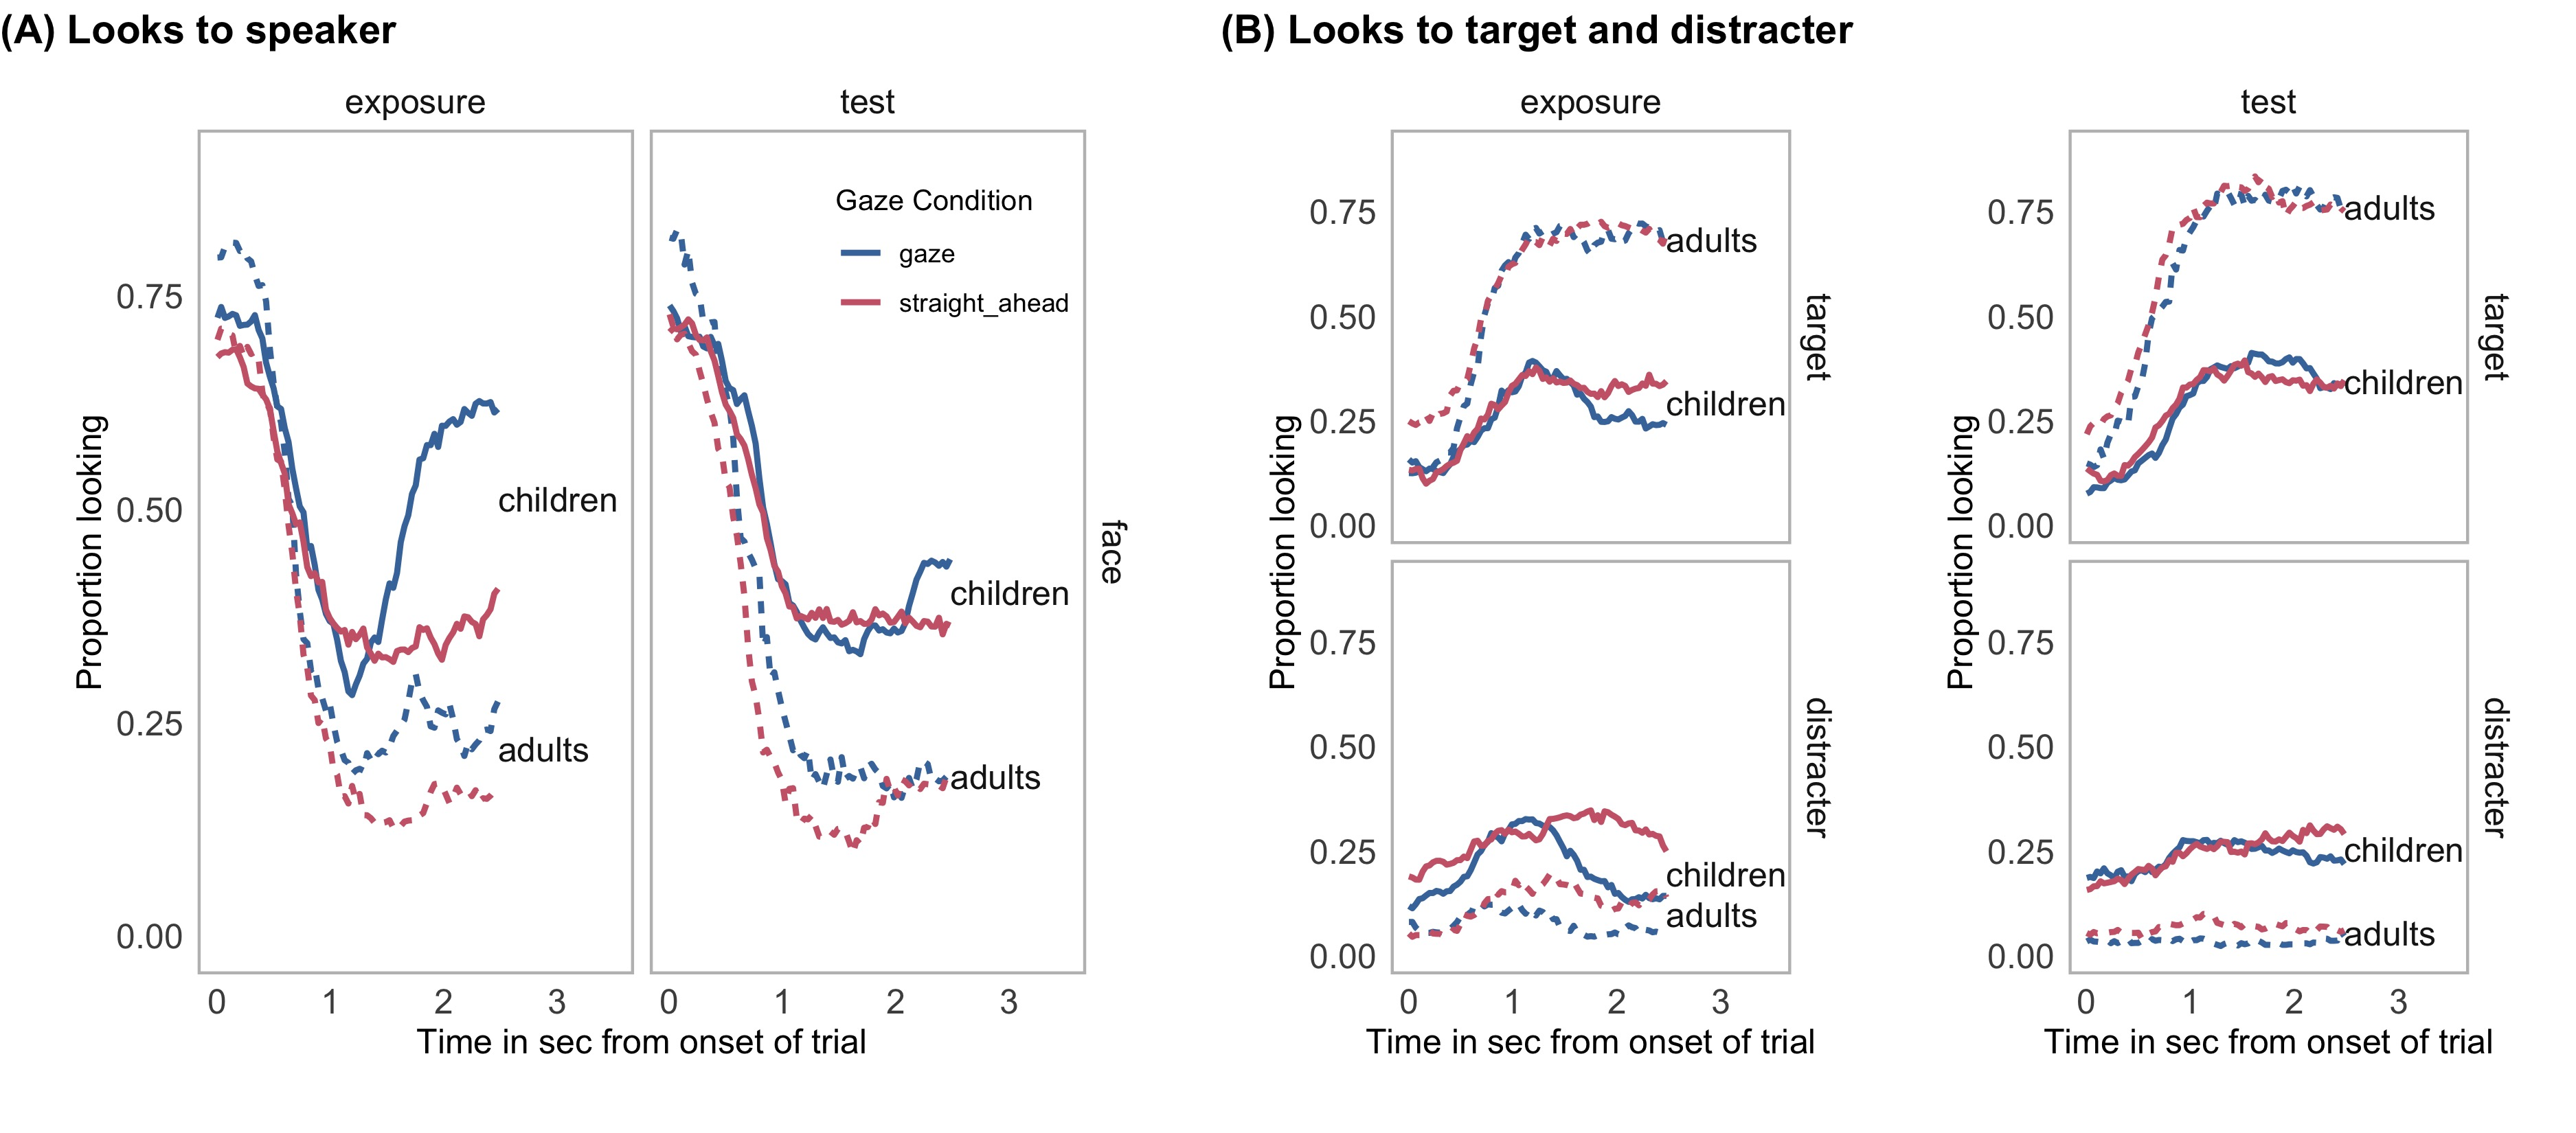
\includegraphics[width=0.85\linewidth]{/Users/kylemacdonald/Documents/Projects/SPEED-ACC-NOVEL/writing/figures/plots/speed_acc_novel_tc} 

}

\caption[Overview of children and adults' looking to the three fixation targets (Speaker, Target, Distracter) over the course of exposure and test trials]{Overview of children and adults' looking to the three fixation targets (Speaker, Target, Distracter) over the course of exposure and test trials. Panel A shows proportion looking to the speaker's face with color indicating gaze condition and line type indicating age group. Panel B shows the same information but for proportion looking to the target and distracter images.}\label{fig:san-tc-plot}
\end{figure*}
\end{CodeChunk}

\emph{Looking to the speaker.} How did the presence of a gaze cue change
learners' decisions to fixate on the speaker? Visual inspection of
Figure \ref{fig:san-tc-plot}A shows that both children and adults tended
to start looking at the speaker at noun onset and shifted their gaze
away as the noun unfolded, with adults doing so sooner compared to
children. On exposure trials when there was a gaze cue, both adults and
children tended to look more to the face at noun onset as indicated by
the higher intercept of the blue curves. Moreover, around one second
after noun onset, listeners tended to shift their attention back to the
speaker's face more often and especially so for children. This pattern
of looking parallels the effect of gaze on children's time course of
fixations while processing familiar words in Experiment 1. On test
trials that were preceded by an exposure trial with gaze, children and
adults tended to look more to the speaker even though there was no gaze
cue present. This pattern suggests that the presence of gaze likely
modulated learners' expectations of gathering disambiguating information
from the speaker on test trials.

\emph{Looking to the target and distracter.} Next, we asked how learners
divided attention between the target and distracter objects. On exposure
trials, looking to both objects increased throughout the trial but more
so for looks to the named object as indicated by the higher asymptote of
the target looking curves. Adults spent more time looking to the target
and less time looking to the distracter as compared to children.
Interestingly, when there was a gaze cue to process, children and adults
allocated fewer fixations to the distracter object, providing evidence
that social information could reduce the potential for learners to
create spurious word-object links during statistical word learning.

\hypertarget{proportion-looking}{%
\subsubsection{Proportion looking}\label{proportion-looking}}

\emph{Learning effects.} Both children (\(M_{gaze}\) = 0.57,
\(M_{no-gaze}\) = 0.55) and adults (\(M_{gaze}\) = 0.91, \(M_{no-gaze}\)
= 0.89) showed evidence of learning the novel word-object links, with
the null value of 0.5 falling below the lower bound of the lowest
credible interval for children's target looking in the No-gaze context
(95\% HDI {[}0.51, 0.60{]}). Our primary question of interest was how
exposure to multiple co-occurrences of word-object pairs would change
learners' distribution of attention between the speaker and objects.
Figure \ref{fig:san-prop-looking-plot} shows proportion looking to the
speaker and the target and distracter objects as a function of trial
number within a word learning block. Both children and adults were more
likely to fixate on the speaker when she provided a gaze cue
(\(\beta_{gaze}\) = 0.09, 95\% HDI {[}0.16, 0.01{]}). Moreover, there
was a developmental difference such that children, but not adults, were
more likely to increase their fixations to the speaker over the course
of the learning block (\(\beta_{age*tr.num}\) = -0.07, 95\% HDI
{[}-0.11, -0.04{]}).

\begin{CodeChunk}
\begin{figure*}[t]

{\centering 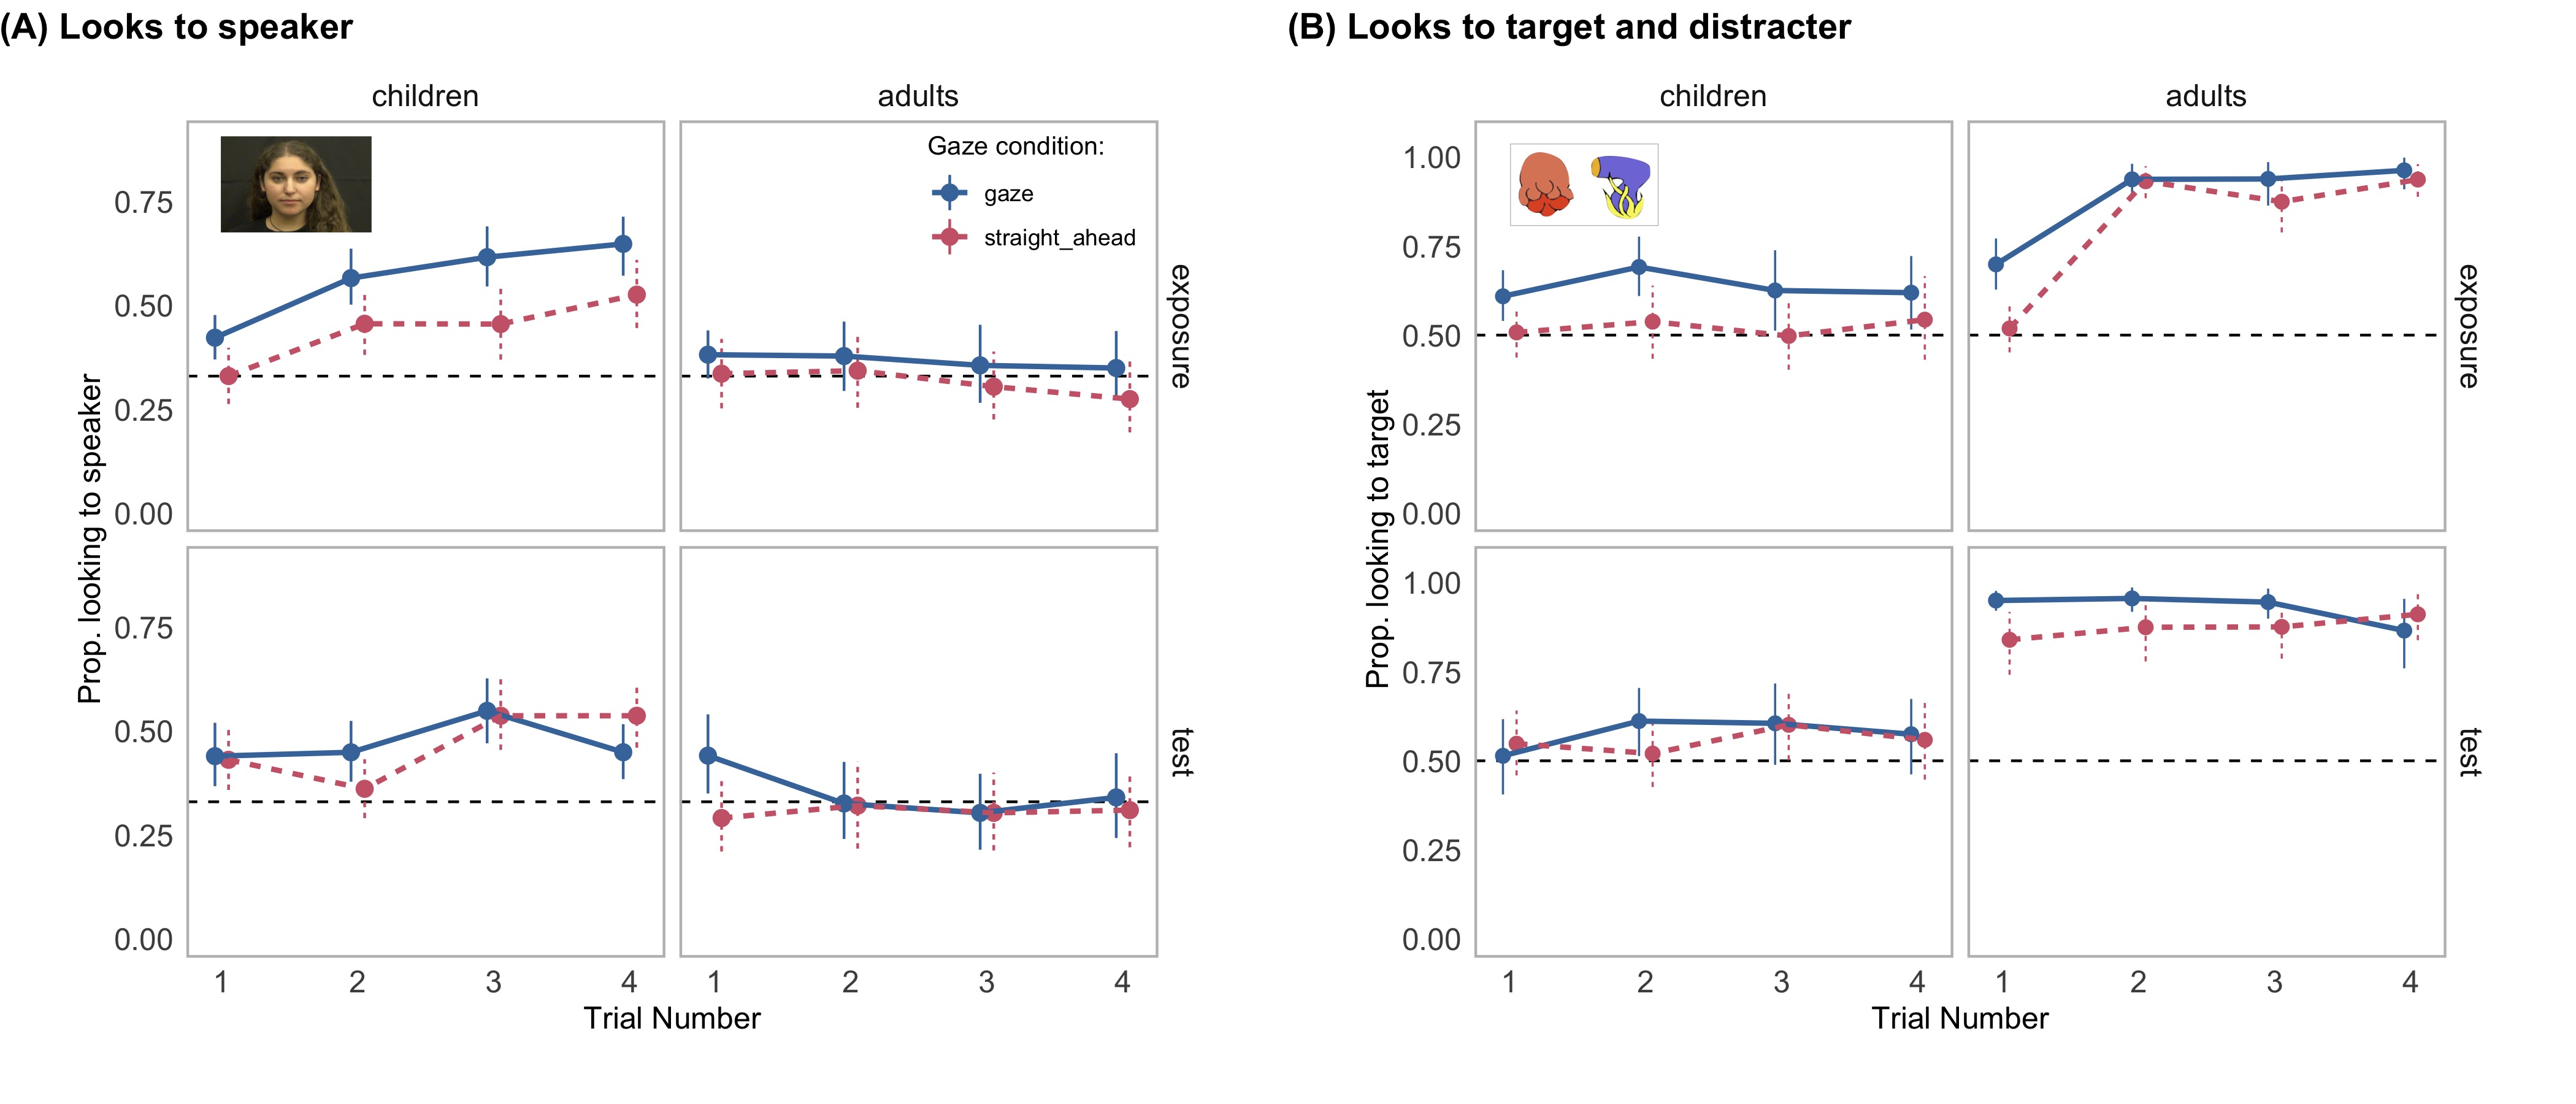
\includegraphics[width=0.85\linewidth]{/Users/kylemacdonald/Documents/Projects/SPEED-ACC-NOVEL/writing/figures/plots/speed_acc_novel_proplook} 

}

\caption[Panel A shows participants’ tendency to look at the speaker on exposure and test trials as a function of the trial number within a learning block]{Panel A shows participants’ tendency to look at the speaker on exposure and test trials as a function of the trial number within a learning block. The horizontal, dashed line represents the tendency to distribute attention equally across the three AOIs. Color indicates gaze condition and error bars represent 95\% credible intervals. Panel B shows the same information but for target and distracter looking across the learning block (left) and aggregated over all trials (right).}\label{fig:san-prop-looking-plot}
\end{figure*}
\end{CodeChunk}

Overall, looking to the target increased as learners were exposed to
more word-object pairings (\(\beta_{tr.num}\) = 0.16, 95\% HDI {[}0.09,
0.24{]}) and was higher when the novel word was accompanied by a gaze
cue (\(\beta_{gaze}\) = 0.14, 95\% HDI {[}0.21, 0.06{]}). Visual
inspection of Figure \ref{fig:san-prop-looking-plot} shows that on the
first exposure trial, both adults and children used the gaze cue to
disambiguate reference, fixating more on the target in the aze
condition. For children, higher target looking on exposure trials with
gaze remained relatively constant across the learning block. In
contrast, adults target looking reached ceiling for both gaze and
no-gaze conditions by trial number two, indicating that they had
successfully used the co-occurrence information across trials to map the
novel word to its referent. We found an interaction between gaze
condition and trial number such that looking to the target increased
more quickly in the No-gaze condition (\(\beta_{gaze*tr.num}\) = 0.02,
95\% HDI {[}0.00, 0.04{]}), which reflects (1) the higher intercept of
target looking in the presence of gaze and (2) rapid learning of the
word-object association via cross-situational information. Finally,
visual inspection of the proportion looking plot suggests that adults
tended to look more the target when learning from a gaze cue, only
reaching similar levels of accuracy in the no-gaze condition at the end
of the learning block. There was not strong evidence for an effect of
the gaze manipulation on children's looking behavior on Test trials.

\emph{Relationship between looking on exposure and test.} For both
children and adults, more time attending to the target object on
exposure trials led to a higher proportion of looking to the target on
test trials, especially for adults (\(\beta_{exposure*age}\) = 0.16,
95\% HDI {[}0.05, 0.28{]}) and as the number of word-object exposures
increased over the course a learning block (\(\beta_{exposure*tr.num}\)
= 0.07, 95\% HDI {[}0.02, 0.12{]}). There was evidence that participants
in the No-gaze condition showed less learning over the course of each
word block (\(\beta_{gaze*tr.num}\) = -0.02, 95\% HDI {[}-0.04,
0.00{]}). This result dovetails with the findings from Experiment 2,
providing evidence that the presence of social information did more than
change attention on exposure trials but instead modulated the
relationship between attention during learning and later memory for
word-object links.

Together, the time course and the proportion looking analyses suggest
that the presence of gaze changed how children and adults allocated
attention while processing novel words. In the context of unfamiliar
objects, children tended to fixate more on a speaker's face when she
provided a post-nominal social cue to reference, a difference in looking
behavior that increased as they were exposed to more word-object
co-occurrences. This result is different from the parallel looking
behavior that we found in Experiment 1 where listeners processed highly
familiar nouns. Moreover, in the presence of a speaker who provided a
gaze cue, children and adults spent less time fixating on the distracter
image, which modulates the word-object connections that learners could
store from labeling event. These changes in gaze patterns, however, did
not generalize to performance differences on Test trials for children.
Finally, as in Experiment 2, we found that the presence of a social cue
increased the strength of the link between attention on exposure and
fixations at test.

\hypertarget{first-shift-rt-and-accuracy}{%
\subsubsection{First shift RT and
Accuracy}\label{first-shift-rt-and-accuracy}}

We next asked how the presence of gaze influenced learners' decision to
stop gathering visual information from the speaker and start fixating on
the novel objects. To quantify the effect the gaze, we fit a Bayesian
linear mixed-effects regression predicting first shift RT as a function
of whether there was a gaze cue present on the trial and age group. Both
children (Gaze \(M_{rt}\) = 1136.7668097 ms, No-gaze \(M_{rt}\) =
878.3664459 ms) and adults (Gaze \(M_{rt}\) = 878.6516854 ms, No-gaze
\(M_{rt}\) = 726.9908386 ms) fixated longer on the speaker when she
provided a gaze cue (\(\beta_{gaze}\) = -0.20, 95\% HDI {[}-0.38,
-0.01{]}). With no evidence of an interaction between gaze condition and
age group (\(\beta_{age*gaze}\) = 0.27, 95\% HDI {[}0.11, 0.44{]}).
Moreover, both (Gaze \(M_{acc}\) = 0.64, No-gaze \(M_{acc}\) = 0.49) and
adults (Gaze \(M_{acc}\) = 0.89, No-gaze \(M_{acc}\) = 0.81) generated
more accurate first shifts in the gaze condition, indicating they were
following the gaze cue on exposure trials (\(\beta_{gaze}\) = -0.57,
95\% HDI {[}-1.13, 0.00{]}).

Finally, we asked whether the presence of gaze affected learning by
predicting first shift accuracy on Test trials. We found that adults
were more accurate than children (\(\beta_{age}\) = 2.24, 95\% HDI
{[}1.50, 3.03{]}), that first shifts became more accurate as learners
experienced repeated exposures to word-object pairings
(\(\beta_{tr.num}\) = 0.21, 95\% HDI {[}-0.02, 0.44{]}). We did not see
evidence for two of our predictions: (1) that children and adults would
generate more accurate first shifts when learning from social gaze
(\(\beta_{gaze}\) = -0.50, 95\% HDI {[}-1.14, 0.14{]}) and (2) that
learning from gaze would modulate the relationship between accuracy over
the course of learning (\(\beta_{gaze*tr.num}\) = -0.30, 95\% HDI
{[}-0.74, 0.12{]}), with the null value falling within each credible
interval.

Returning to our three behavioral predictions. First, we found evidence
that the gaze cue changed learners' decisions about how to distribute
visual attention. Both children and adults spent more time fixating on a
speaker when she provided a useful social cue to reference. This shift
in looking led to fewer looks to the objects overall, with a higher
proportion of those fixations allocated to the named object and less
looking to the other objects in the scene.

Second, both children and adults changed how they distributed attention
across the speaker and objects throughout learning. In line with our
prediction, adults decreased the amount of time fixating on the speaker
as they gained more exposures to the word-object pairings, suggesting
that they shifted gaze patterns to seek visual information that
supported strengthening associations between words and objects.
Children, however, showed the opposite pattern, increasing their
fixations to the speaker throughout accumulating statistical
information. This developmental difference suggests that increasing
fixations to the social partner may have been more useful for children's
who were still trying to disambiguate the novel words; whereas adults,
who showed evidence of successful disambiguation after the second
exposure trial, did not prioritize fixating on the speaker to gather
disambiguating information and could focus attention on the objects
instead.

Third, we found mixed evidence that the presence of gaze modulated the
relationship between visual attention during labeling and learning of
the novel word-object mappings. Both children and adults generated a
higher proportion of shifts landing on the target when there was
post-nominal gaze cue available. But only adults spent more time
fixating on the target object and generated more accurate first shifts
for word-object links learned in the presence of gaze. And, on both
measures of learning, children showed relatively weak evidence of
learning the novel word-object links overall, which could have masked
the effects of seeking social information on exposure trials.

\hypertarget{general-discussion}{%
\section{General Discussion}\label{general-discussion}}

During grounded language processing, gathering visual information from a
social partner can facilitate comprehension and learning. Do children
integrate prior knowledge of words when deciding to seek social
information? And how does children's social information seeking change
as they build more stable connections between words and concepts? In
this work, we pursued the idea that learners flexibly adjust their eye
movements to gather social gaze when it was useful for their
comprehension. We presented evidence for this explanation by tracking
children and adults' eye movements as they processed familiar and novel
words accompanied by a gaze cue. We also measured how learners' gaze
dynamics changed as they accumulated cross-situational statistical
information about novel word-object links.

In Experiment 1, children and adults shifted attention away from the
speaker's face before gathering a post-nominal gaze cue while processing
familiar words. Experiment 2 showed that the presence of gaze in the
context of processing novel words increased adults' fixations to a
social target relative to objects, focused attention on a single object,
and modulated the strength of the relationship between visual attention
during labeling and learning of word-object pairings. Finally, in
Experiment 2, both children and adults fixated more on a speaker to seek
a post-nominal gaze cue while processing novel words. This delay
resulted in more attention allocated to the target object and less
looking to the distracter object during labeling, an effect that
increased over the course of the task for children. Moreover, adults,
but not children, showed evidence of stronger learning in the presence
of social gaze while both age groups were capable of learning the
word-object pairings from cross-situational statistics without gaze.

How should we characterize the effects of gaze on information seeking
and word learning in our task? In sum, these results suggest that
listeners can adapt to seek social information that supports language
processing, but they may integrate their uncertainty over the
word-object links when deciding to do so. Moreover, seeking gaze changes
how learners distribute attention across the objects such that looking
to the focus of a speaker's gaze increases while fixations to the other
objects decrease. This pattern of looking generalized to test trials
where there was not a gaze cue present, showing how social gaze effects
could accumulate, thus modulating the information that comes into
contact with children's statistical learning mechanisms. Finally,
seeking a social gaze cue increased the strength of the relationship
between fixations during learning and performance at test, suggesting
that learners were getting more information out of each fixation when it
was directed by social gaze. This finding dovetails with other empirical
work showing that the presence of social information changes how
children extract and store new information (Wu et al. 2011; Cleveland,
Schug, and Striano 2007; Yoon, Johnson, and Csibra 2008).

\hypertarget{limitations}{%
\subsection{Limitations}\label{limitations}}

This work has several limitations. First, we did not see evidence that
the effects of seeking social gaze generalized to contexts without gaze
(i.e., learning) in Experiment 2. Moreover, children did not show
evidence of strong uptake of the novel word-object links overall. In
future work, we will modify our social, cross-situational word learning
paradigm to increase learning and better detect any effects of seeking
social information. For example, Yurovsky, Wade, and Frank (2013) found
that 3-5 year-olds show stronger word learning from an extended, as
opposed to brief, social cue to reference. Following this work, we could
increase the length of the gaze cue, which was relatively short in these
studies (\textasciitilde{}2 sec). Moreover, we will modify the test
trials to use the two newly learned objects. This change should remove
any novelty preference that may have pushed children to allocate
attention to the unfamiliar distracter object that children saw for the
first time (Houston-Price and Nakai 2004).

Second, while our paradigm measured the effect of social cues on
information selection across multiple labeling events, this is still a
much shorter timescale and a smaller number of exposures relative to
children's actual language input. Moreover, the visual world paradigm,
while well-controlled, is highly constrained relative to the complexity
of children's information seeking decisions in naturalistic learning
environments. A valuable next step would be to use head-mounted cameras
and eye trackers that allow for measurement of where children choose to
look during everyday social interactions. It would be interesting to
know how the rate of children's social referencing changes when
encountering new objects/words at both discourse and developmental
timescales. To link our lab-based findings to natural behavior will
require a shift to observational studies of child-caregiver interactions
in the home environment (see Sanchez et al. (2018) for an example of
this approach).

Third, we used a binary manipulation of the social context -- a fully
disambiguating gaze cue or entirely ambiguous label without a gaze cue.
These extremes do not reflect the complexity of children's input from
social interactions. That is, observational studies of child-caregiver
play sessions show that social cues such as eye gaze or pointing are
noisy (Frank, Tenenbaum, and Fernald 2013) and that caregivers tend to
provide a mixture of ambiguous and clear labeling events (Medina et al.
2011; Yurovsky, Smith, and Yu 2013). Moreover, our prior work suggests
that adults are sensitive to the graded changes in the strength of a
speaker's gaze cue, storing word-object links with greater fidelity when
they expected the gaze cue to be reliable (MacDonald, Yurovsky, and
Frank 2017). It would be interesting to know how children's real-time
information selection responds to continuous changes in the utility of
social information for reducing referential ambiguity. This modification
would also allow us to measure whether children are building
expectations about the usefulness of seeking information from specific
people, which seems important since observational work shows large
individual and cultural differences in the proportion of unambiguous
naming episodes across parent-child dyads (i.e., accommodation of the
conversation to the child) (Cartmill et al. 2013; Fernald 2010).

\hypertarget{conclusions}{%
\subsection{Conclusions}\label{conclusions}}

In this paper, we presented a set of empirical studies that integrated
social-pragmatic and statistical accounts of language acquisition with
ideas from goal-based accounts of vision. We found that listeners'
decisions to seek social information varied depending on their
uncertainty over word-object mappings. In the context of processing
novel, but not familiar words, listeners adapted their gaze to seek a
post-nominal social cue to reference. This behavior led to increased
visual attention to a single object and less attention distributed
across potential spurious word-object links. Moreover, following gaze
modulated the relationship between learners' real-time looking behavior
during labeling and their learning of novel words. More generally, the
approach taken in this work sheds light on how children can integrate
social and statistical information when deploying eye movements to
gather information during language processing, which, in turn, shapes
the information that comes into contact with their statistical learning
mechanisms.

\vspace{1em}

\fbox{\parbox[b][][c]{7.3cm}{\centering All data and code for this paper are available at\\\url{https://github.com/kemacdonald/speed-acc-novel/tree/master/writing/san-cogsci-2019}}}
\vspace{1em}

\hypertarget{acknowledgements}{%
\section{Acknowledgements}\label{acknowledgements}}

We are grateful to the people who participated in this research. Thanks
to Kayla Constandse, Tami Alade, and Hannah Slater for help with data
collection. This work was supported by an NSF GRFP to KM and a Jacobs
Foundation Fellowship to MCF.

\hypertarget{references}{%
\section{References}\label{references}}

\setlength{\parindent}{-0.1in} 
\setlength{\leftskip}{0.125in}

\noindent

\hypertarget{refs}{}
\leavevmode\hypertarget{ref-allopenna1998tracking}{}%
Allopenna, Paul D, James S Magnuson, and Michael K Tanenhaus. 1998.
``Tracking the Time Course of Spoken Word Recognition Using Eye
Movements: Evidence for Continuous Mapping Models.'' \emph{Journal of
Memory and Language} 38 (4). Elsevier: 419--39.

\leavevmode\hypertarget{ref-baldwin1993infants}{}%
Baldwin, Dare A. 1993. ``Infants' Ability to Consult the Speaker for
Clues to Word Reference.'' \emph{Journal of Child Language} 20 (02).
Cambridge Univ Press: 395--418.

\leavevmode\hypertarget{ref-bloom2002children}{}%
Bloom, Paul. 2002. \emph{How Children Learn the Meaning of Words}. The
MIT Press.

\leavevmode\hypertarget{ref-blythe2016word}{}%
Blythe, Richard A, Andrew DM Smith, and Kenny Smith. 2016. ``Word
Learning Under Infinite Uncertainty.'' \emph{Cognition} 151. Elsevier:
18--27.

\leavevmode\hypertarget{ref-blythe2010learning}{}%
Blythe, Richard A, Kenny Smith, and Andrew DM Smith. 2010. ``Learning
Times for Large Lexicons Through Cross-Situational Learning.''
\emph{Cognitive Science} 34 (4). Wiley Online Library: 620--42.

\leavevmode\hypertarget{ref-brooks2005development}{}%
Brooks, Rechele, and Andrew N Meltzoff. 2005. ``The Development of Gaze
Following and Its Relation to Language.'' \emph{Developmental Science} 8
(6). Wiley Online Library: 535--43.

\leavevmode\hypertarget{ref-burkner2017brms}{}%
Bürkner, Paul-Christian. 2017. ``Brms: An R Package for Bayesian
Multilevel Models Using Stan.'' \emph{Journal of Statistical Software}
80 (1). Foundation for Open Access Statistics: 1--28.

\leavevmode\hypertarget{ref-carpenter1998social}{}%
Carpenter, Malinda, Katherine Nagell, Michael Tomasello, George
Butterworth, and Chris Moore. 1998. ``Social Cognition, Joint Attention,
and Communicative Competence from 9 to 15 Months of Age.''
\emph{Monographs of the Society for Research in Child Development}.
JSTOR, i--174.

\leavevmode\hypertarget{ref-cartmill2013quality}{}%
Cartmill, Erica A, Benjamin F Armstrong, Lila R Gleitman, Susan
Goldin-Meadow, Tamara N Medina, and John C Trueswell. 2013. ``Quality of
Early Parent Input Predicts Child Vocabulary 3 Years Later.''
\emph{Proceedings of the National Academy of Sciences} 110 (28).
National Acad Sciences: 11278--83.

\leavevmode\hypertarget{ref-castro2009human}{}%
Castro, Rui M, Charles Kalish, Robert Nowak, Ruichen Qian, Tim Rogers,
and Xiaojin Zhu. 2009. ``Human Active Learning.'' In \emph{Advances in
Neural Information Processing Systems}, 241--48.

\leavevmode\hypertarget{ref-clark2009first}{}%
Clark, Eve V. 2009. \emph{First Language Acquisition}. Cambridge
University Press.

\leavevmode\hypertarget{ref-cleveland2007joint}{}%
Cleveland, Allison, Mariah Schug, and Tricia Striano. 2007. ``Joint
Attention and Object Learning in 5-and 7-Month-Old Infants.''
\emph{Infant and Child Development} 16 (3). Wiley Online Library:
295--306.

\leavevmode\hypertarget{ref-estigarribia2007getting}{}%
Estigarribia, Bruno, and Eve V Clark. 2007. ``Getting and Maintaining
Attention in Talk to Young Children.'' \emph{Journal of Child Language}
34 (4). Cambridge University Press: 799--814.

\leavevmode\hypertarget{ref-fernald2010getting}{}%
Fernald, Anne. 2010. ``Getting Beyond the `Convenience Sample' in
Research on Early Cognitive Development.'' \emph{Behavioral and Brain
Sciences} 33 (2-3). Cambridge University Press: 91--92.

\leavevmode\hypertarget{ref-frank2009using}{}%
Frank, Michael C, Noah D Goodman, and Joshua B Tenenbaum. 2009. ``Using
Speakers' Referential Intentions to Model Early Cross-Situational Word
Learning.'' \emph{Psychological Science} 20 (5). SAGE Publications:
578--85.

\leavevmode\hypertarget{ref-frank2013social}{}%
Frank, Michael C, Joshua B Tenenbaum, and Anne Fernald. 2013. ``Social
and Discourse Contributions to the Determination of Reference in
Cross-Situational Word Learning.'' \emph{Language Learning and
Development} 9 (1). Taylor \&amp; Francis: 1--24.

\leavevmode\hypertarget{ref-gureckis2012self}{}%
Gureckis, Todd M, and Douglas B Markant. 2012. ``Self-Directed Learning
a Cognitive and Computational Perspective.'' \emph{Perspectives on
Psychological Science} 7 (5). Sage Publications: 464--81.

\leavevmode\hypertarget{ref-hayhoe2005eye}{}%
Hayhoe, Mary, and Dana Ballard. 2005. ``Eye Movements in Natural
Behavior.'' \emph{Trends in Cognitive Sciences} 9 (4). Elsevier:
188--94.

\leavevmode\hypertarget{ref-hidaka2017quantifying}{}%
Hidaka, Shohei, Takuma Torii, and George Kachergis. 2017. ``Quantifying
the Impact of Active Choice in Word Learning.'' In. Cognitive Science
Society.

\leavevmode\hypertarget{ref-hollich2000breaking}{}%
Hollich, George J, Kathy Hirsh-Pasek, Roberta Michnick Golinkoff,
Rebecca J Brand, Ellie Brown, He Len Chung, Elizabeth Hennon, Camille
Rocroi, and Lois Bloom. 2000. ``Breaking the Language Barrier: An
Emergentist Coalition Model for the Origins of Word Learning.''
\emph{Monographs of the Society for Research in Child Development}.
JSTOR, i--135.

\leavevmode\hypertarget{ref-houston2004distinguishing}{}%
Houston-Price, Carmel, and Satsuki Nakai. 2004. ``Distinguishing Novelty
and Familiarity Effects in Infant Preference Procedures.'' \emph{Infant
and Child Development: An International Journal of Research and
Practice} 13 (4). Wiley Online Library: 341--48.

\leavevmode\hypertarget{ref-kachergis2013actively}{}%
Kachergis, George, Chen Yu, and Richard M Shiffrin. 2013. ``Actively
Learning Object Names Across Ambiguous Situations.'' \emph{Topics in
Cognitive Science} 5 (1). Wiley Online Library: 200--213.

\leavevmode\hypertarget{ref-macdonald2018speed}{}%
MacDonald, Kyle, Virginia Marchman, Anne Fernald, and Michael C Frank.
2018. ``Children Seek Visual Information During Signed and Spoken
Language Comprehension.'' \emph{Preprint PsyArXiv}.

\leavevmode\hypertarget{ref-macdonald2017social}{}%
MacDonald, Kyle, Daniel Yurovsky, and Michael C Frank. 2017. ``Social
Cues Modulate the Representations Underlying Cross-Situational
Learning.'' \emph{Cognitive Psychology} 94. Elsevier: 67--84.

\leavevmode\hypertarget{ref-maris2007nonparametric}{}%
Maris, Eric, and Robert Oostenveld. 2007. ``Nonparametric Statistical
Testing of Eeg-and Meg-Data.'' \emph{Journal of Neuroscience Methods}
164 (1). Elsevier: 177--90.

\leavevmode\hypertarget{ref-mcmurray2012word}{}%
McMurray, Bob, Jessica S Horst, and Larissa K Samuelson. 2012. ``Word
Learning Emerges from the Interaction of Online Referent Selection and
Slow Associative Learning.'' \emph{Psychological Review} 119 (4).
American Psychological Association: 831.

\leavevmode\hypertarget{ref-medina2011words}{}%
Medina, Tamara Nicol, Jesse Snedeker, John C Trueswell, and Lila R
Gleitman. 2011. ``How Words Can and Cannot Be Learned by Observation.''
\emph{Proceedings of the National Academy of Sciences} 108 (22).
National Acad Sciences: 9014--9.

\leavevmode\hypertarget{ref-partridge2015young}{}%
Partridge, Eric, Matthew G McGovern, Amanda Yung, and Celeste Kidd.
2015. ``Young Children's Self-Directed Information Gathering on
Touchscreens.'' In \emph{Proceedings of the 37th Annual Conference of
the Cognitive Science Society}.

\leavevmode\hypertarget{ref-quine19600}{}%
Quine, Willard V. 1960. ``0. Word and Object.'' \emph{111e MIT Press}.

\leavevmode\hypertarget{ref-roy2002learning}{}%
Roy, Deb K, and Alex P Pentland. 2002. ``Learning Words from Sights and
Sounds: A Computational Model.'' \emph{Cognitive Science} 26 (1). Wiley
Online Library: 113--46.

\leavevmode\hypertarget{ref-sanchez2018postural}{}%
Sanchez, Alessandro, Bria Long, Allison M Kraus, and Michael C Frank.
2018. ``Postural Developments Modulate Children's Visual Access to
Social Information.'' PsyArXiv.

\leavevmode\hypertarget{ref-sekicki2018eye}{}%
Sekicki, Mirjana, and Maria Staudte. 2018. ``Eye'll Help You Out! How
the Gaze Cue Reduces the Cognitive Load Required for Reference
Processing.'' \emph{Cognitive Science}. Wiley Online Library.

\leavevmode\hypertarget{ref-settles2012active}{}%
Settles, Burr. 2012. ``Active Learning.'' \emph{Synthesis Lectures on
Artificial Intelligence and Machine Learning} 6 (1). Morgan \& Claypool
Publishers: 1--114.

\leavevmode\hypertarget{ref-siskind1996computational}{}%
Siskind, Jeffrey Mark. 1996. ``A Computational Study of
Cross-Situational Techniques for Learning Word-to-Meaning Mappings.''
\emph{Cognition} 61 (1). Elsevier: 39--91.

\leavevmode\hypertarget{ref-smith2008infants}{}%
Smith, Linda B, and Chen Yu. 2008. ``Infants Rapidly Learn Word-Referent
Mappings via Cross-Situational Statistics.'' \emph{Cognition} 106 (3).
Elsevier: 1558--68.

\leavevmode\hypertarget{ref-smith2013visual}{}%
---------. 2013. ``Visual Attention Is Not Enough: Individual
Differences in Statistical Word-Referent Learning in Infants.''
\emph{Language Learning and Development} 9 (1). Taylor \& Francis:
25--49.

\leavevmode\hypertarget{ref-wu2011infants}{}%
Wu, Rachel, Alison Gopnik, Daniel C Richardson, and Natasha Z Kirkham.
2011. ``Infants Learn About Objects from Statistics and People.''
\emph{Developmental Psychology} 47 (5). American Psychological
Association: 1220.

\leavevmode\hypertarget{ref-yoon2008communication}{}%
Yoon, Jennifer MD, Mark H Johnson, and Gergely Csibra. 2008.
``Communication-Induced Memory Biases in Preverbal Infants.''
\emph{Proceedings of the National Academy of Sciences} 105 (36).
National Acad Sciences: 13690--5.

\leavevmode\hypertarget{ref-yu2007unified}{}%
Yu, Chen, and Dana H Ballard. 2007. ``A Unified Model of Early Word
Learning: Integrating Statistical and Social Cues.''
\emph{Neurocomputing} 70 (13). Elsevier: 2149--65.

\leavevmode\hypertarget{ref-yu2007rapid}{}%
Yu, Chen, and Linda B Smith. 2007. ``Rapid Word Learning Under
Uncertainty via Cross-Situational Statistics.'' \emph{Psychological
Science} 18 (5). SAGE Publications: 414--20.

\leavevmode\hypertarget{ref-yu2012embodied}{}%
---------. 2012. ``Embodied Attention and Word Learning by Toddlers.''
\emph{Cognition}. Elsevier.

\leavevmode\hypertarget{ref-yu2016social}{}%
---------. 2016. ``The Social Origins of Sustained Attention in
One-Year-Old Human Infants.'' \emph{Current Biology} 26 (9). Elsevier:
1235--40.

\leavevmode\hypertarget{ref-yurovsky2013statistical}{}%
Yurovsky, Daniel, Linda B Smith, and Chen Yu. 2013. ``Statistical Word
Learning at Scale: The Baby's View Is Better.'' \emph{Developmental
Science} 16 (6). Wiley Online Library: 959--66.

\leavevmode\hypertarget{ref-yurovsky2013online}{}%
Yurovsky, Daniel, Anna Wade, and Michael Frank. 2013. ``Online
Processing of Speech and Social Information in Early Word Learning.'' In
\emph{Proceedings of the Annual Meeting of the Cognitive Science
Society}. Vol. 35. 35.

\bibliographystyle{apacite}


\end{document}
